\section{Admin}
\subsection{Dashboard}
Trang dashboard của Admin đượcthiết kế để theo dõi và quản lý hiệu suất hệ thống, phân tích dữ liệu người dùng trong hệ thống học trực tuyến.
\begin{itemize}
    \item Hiệu suất hệ thống: FCP, LCP INP
    \item Số liệu tổng quan của hệ thống
    \begin{figure}[H]
        \centering
        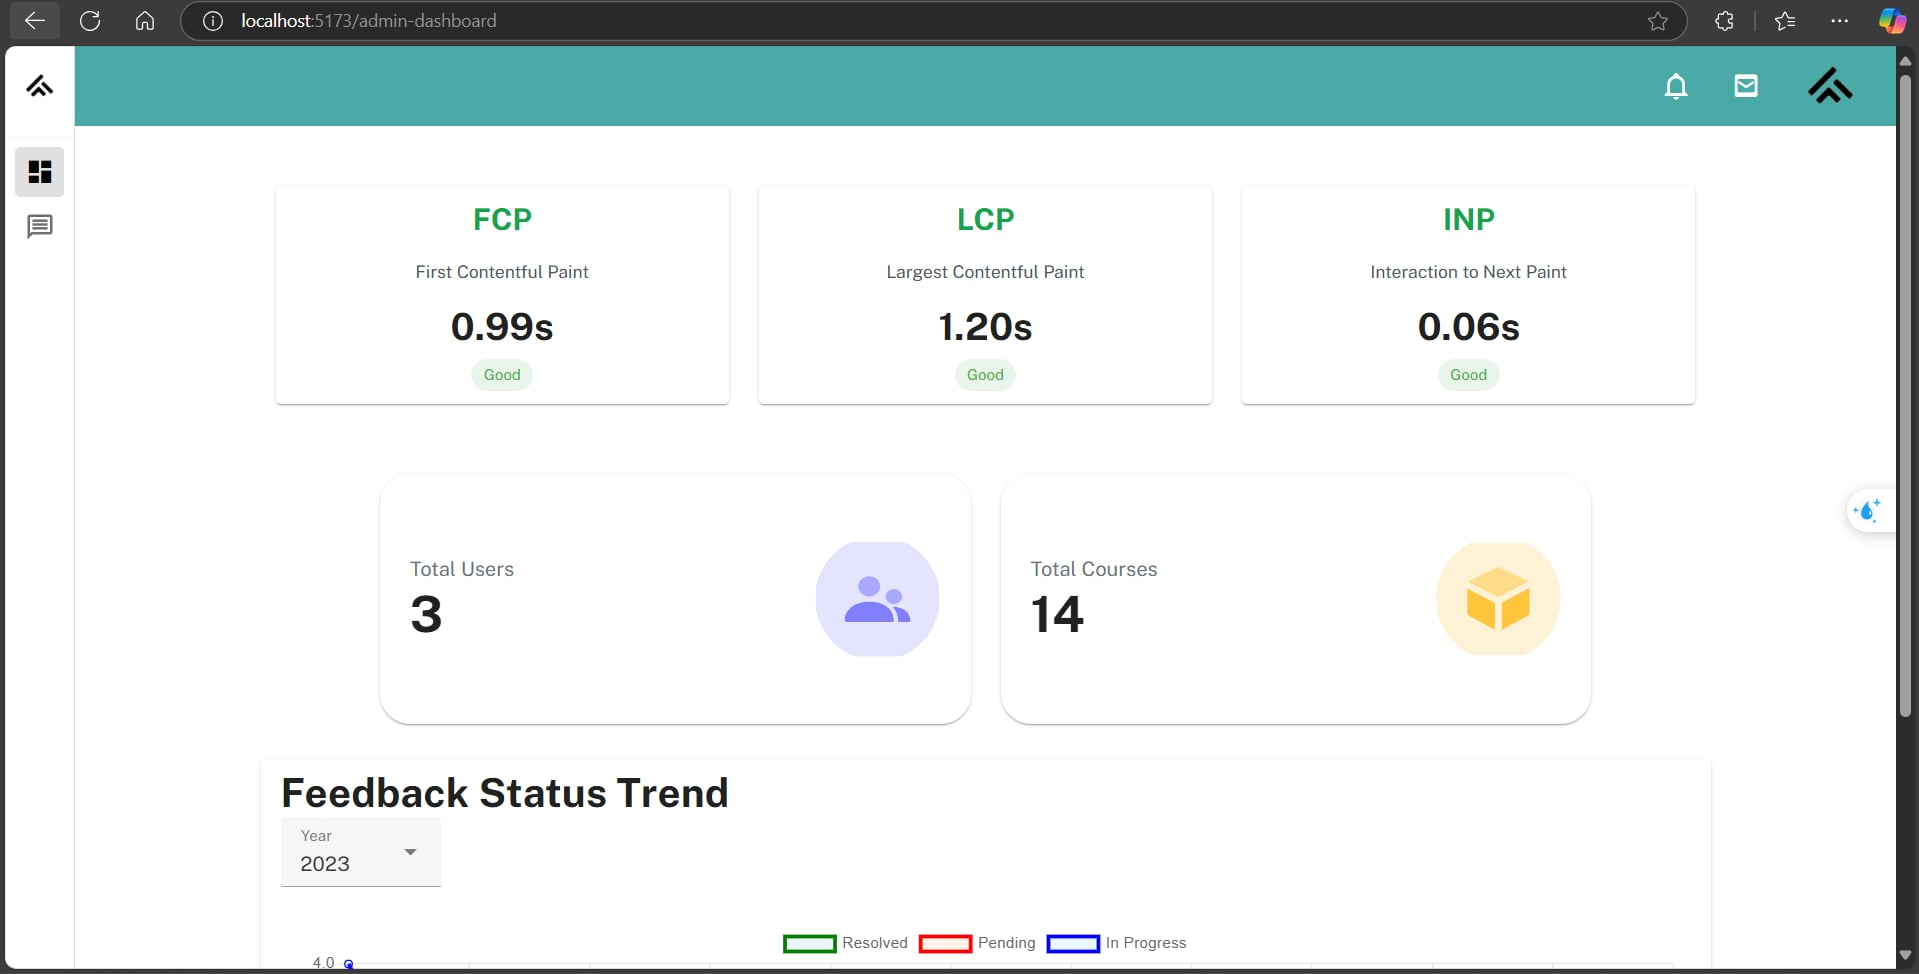
\includegraphics[width=0.8\linewidth]{images/dashboard_stat.png}
        \caption{Dashboard Admin}
        \label{fig:enter-label}
    \end{figure}
    \item Biểu đồ thống kê feedback: đã giải quyết, đang xử lí, đang chờ
    \begin{figure}[H]
        \centering
        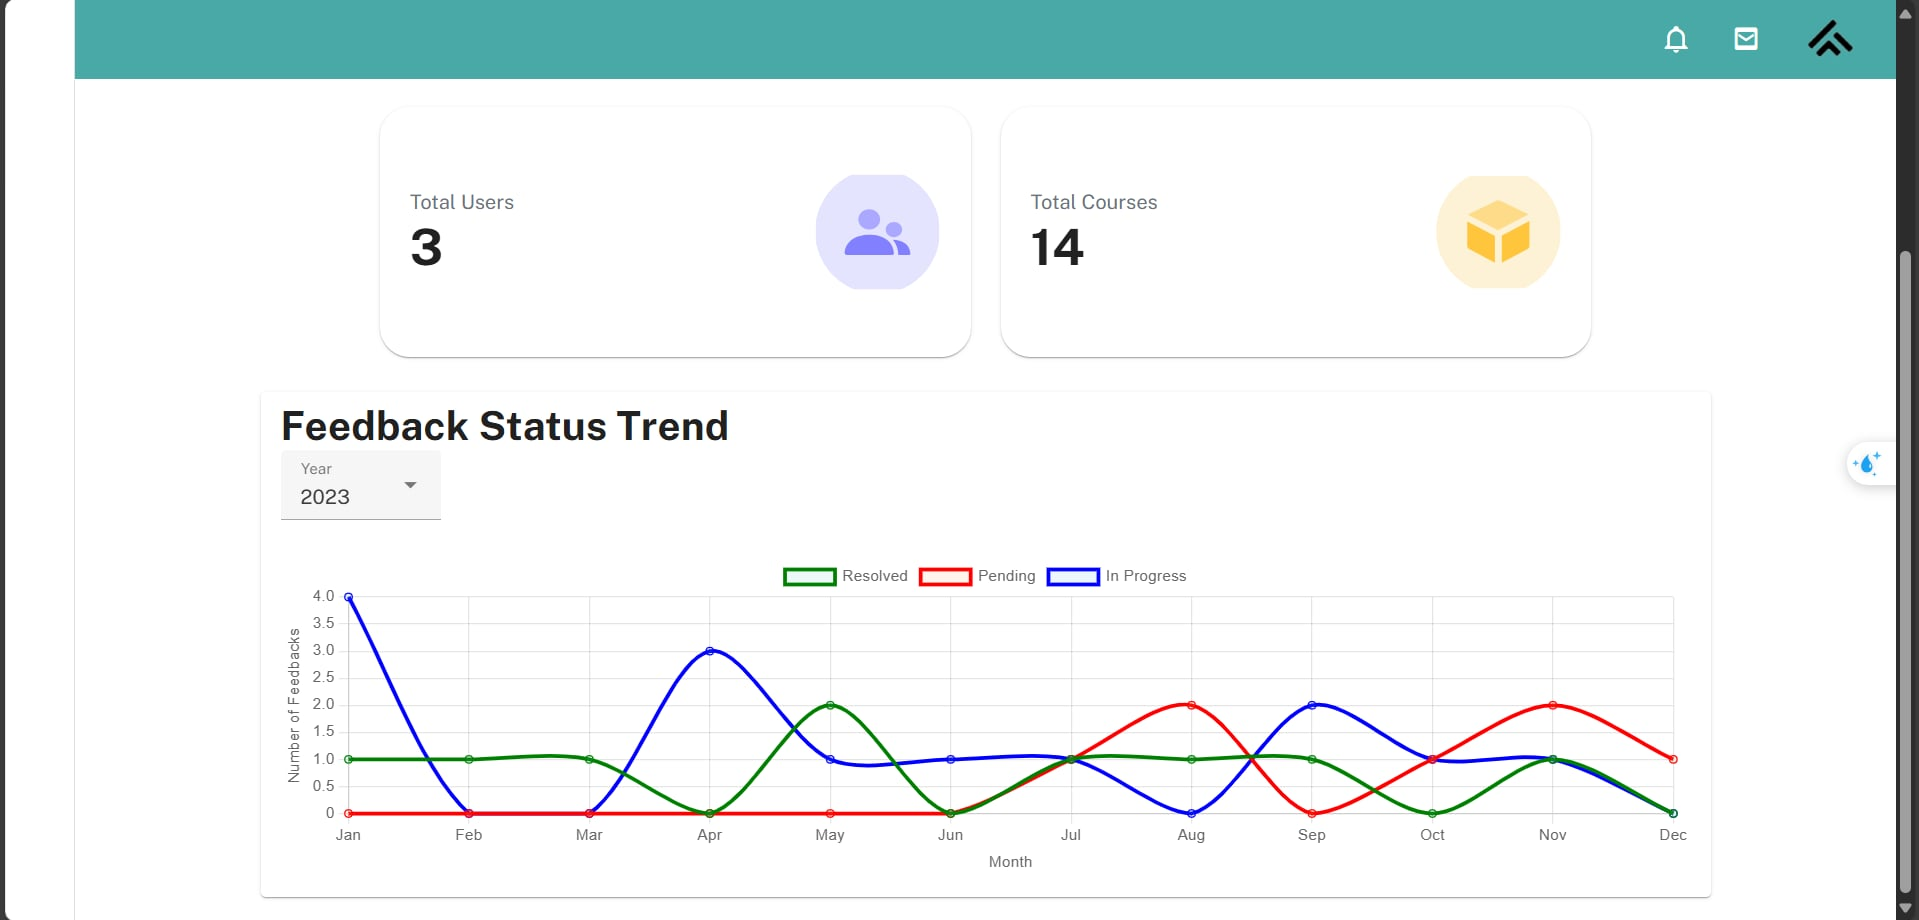
\includegraphics[width=0.8\linewidth]{images/dashboard_feedback.png}
        \caption{Biểu đồ thống kê feedback}
        \label{fig:enter-label}
    \end{figure}
\end{itemize}
\subsection{Feedback Management}
Admin có thể theo dõi và xử lý các phản hồi (feedback) từ người dùng thông qua một bảng danh sách hiển thị chi tiết từng feedback. Mỗi phản hồi bao gồm các thông tin chính như:
\begin{itemize}
    \item Người gửi (User): Tên hoặc ID của người dùng đã gửi phản hồi.
    \item Tiêu đề phản hồi, mô tả
    \item Phân loại:
    \begin{itemize}
        \item Performance
        \item Bug Report
        \item Feature Request
        \item UI/UX
        \item Others
    \end{itemize}
    \item Rating: 1-5 sao
    \item Trạng thái feedback
\end{itemize}

\begin{figure}[H]
        \centering
        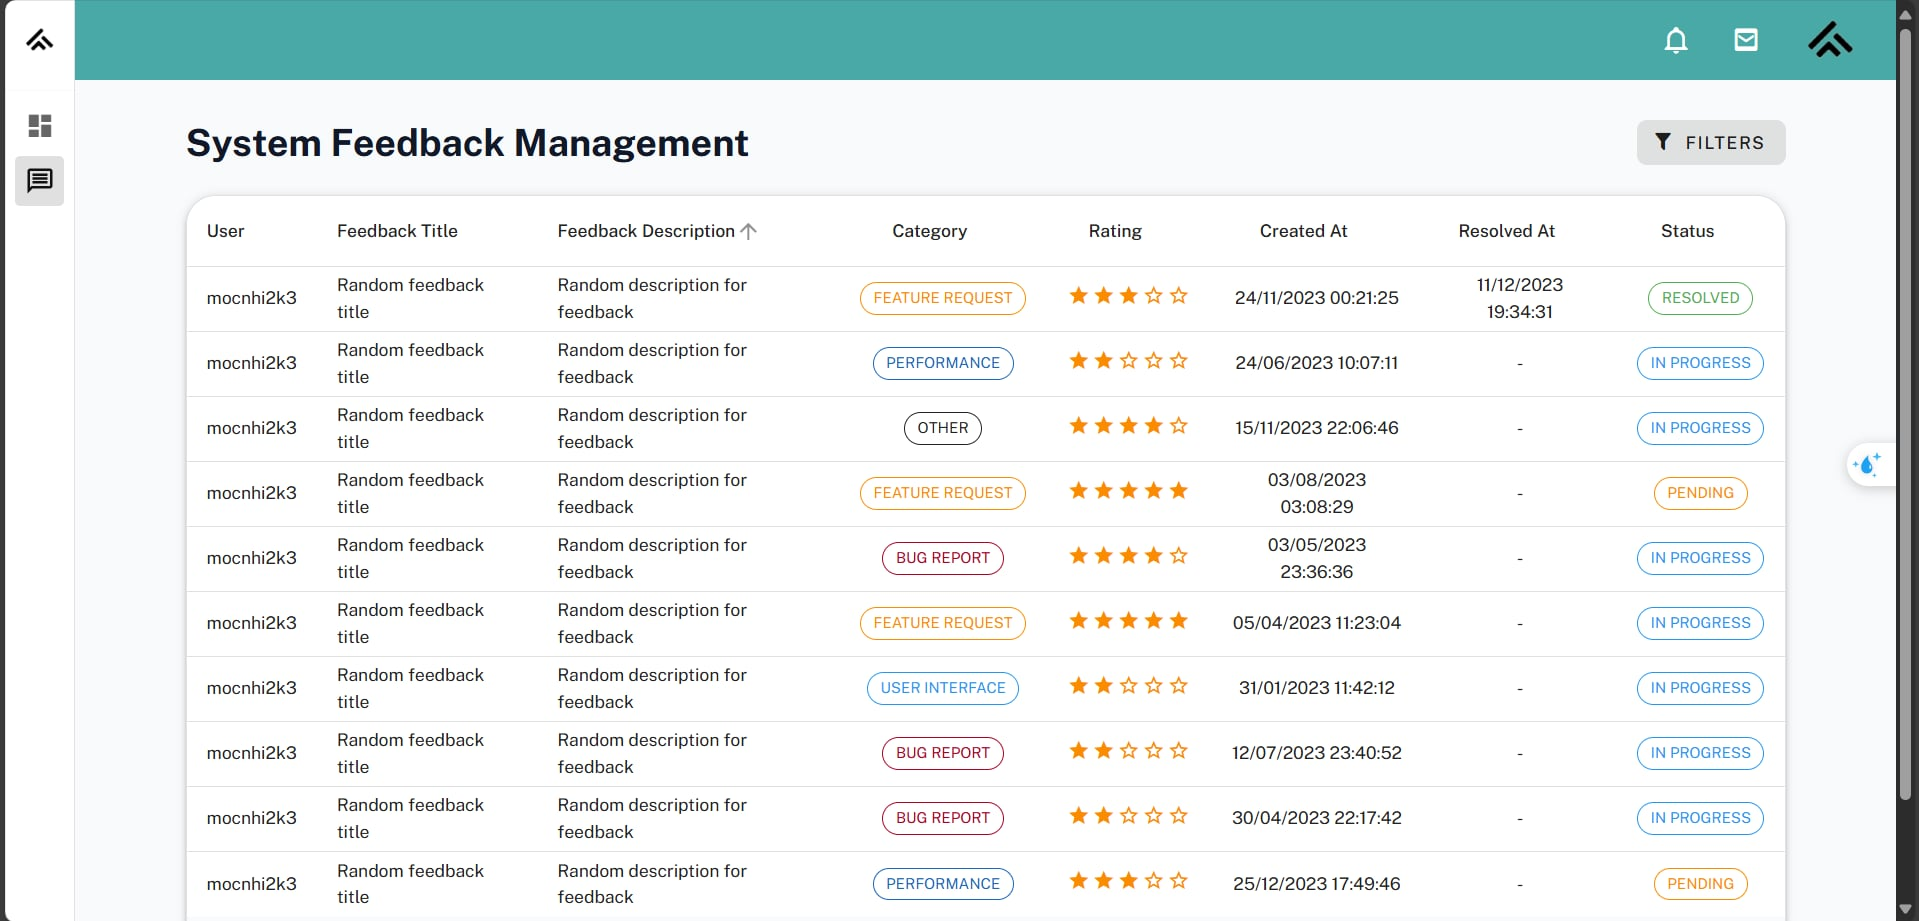
\includegraphics[width=0.8\linewidth]{images/feedback_management.png}
        \caption{Danh sách feedback của hệ thống}
        \label{fig:enter-label}
    \end{figure}
Admin có thể lọc và tìm kiếm các phản hồi dựa trên:
\begin{itemize}
    \item Khoảng thời gian nhất định.
    \item Lọc theo phân loại.
    \item Lọc theo trạng thái feedback.
\end{itemize}
\begin{figure}[H]
        \centering
        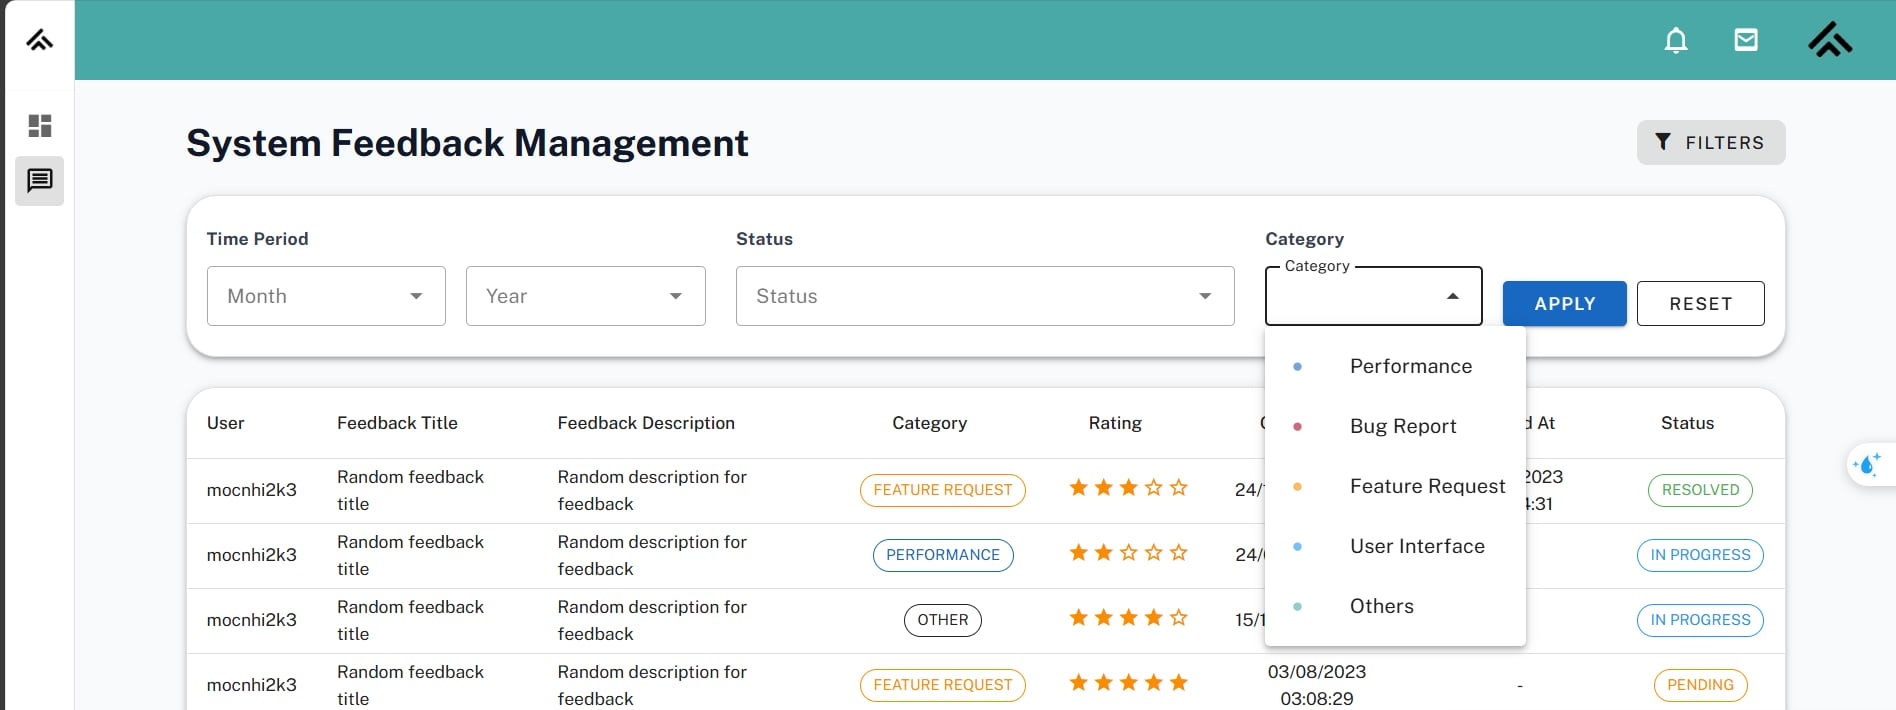
\includegraphics[width=0.8\linewidth]{images/feedback_filter.png}
        \caption{Lọc danh sách feedback}
        \label{fig:enter-label}
    \end{figure}